\chapter{Teil B}
\label{cha:TeilB}
Im Folgenden wird Teil B dieser Arbeit behandelt. Bei embedded-Linux Systemen mit höherer Leistung und vor allem einer dedizierten Grafikkarte, die es sogar ermöglicht 3D Beschleunigung in Hardware oder Full-HD Anzeige mittels HDMI-Monitoren, ist die Frage nicht, ob ein Display angeschlossen werden kann, sondern eher welches. Die HDMI-Schnittstelle bietet bereits die Möglichkeit eine Vielzahl von Anzeigegeräten anzuschließen. Befindet man sich allerdings im embedded Bereich, so sind die Anforderungen an die Kompaktheit der Baugröße, oft von sehr großer Bedeutung. Zu diesem Zweck wurde in Teil B dieser Arbeit eine Möglichkeit entwickelt, die den Anschluss von ausgewählten Displays mit einem Formfaktor von 7"' bei der Auflösung von 800x480 mit RGB- sowie LVDS-Schnittstelle auf kompaktem Raum mit dem HDMI-Anschluss des embedded-Boards verbinden lässt. Betrachtet man die entwickelte Hardware näher, wird klar, dass diese mit jeder erdenklichen HDMI-Quelle verwendbar ist und im weitesten Sinne einen kompakten HDMI-Monitor darstellt.
In den nachfolgenden Kapiteln werden die Konzeption sowie die entwickelte Hard- und Software behandelt. Im Anschluss folgt ein Kapitel, welches die bekannten Fehler im Projekt aufzeigt.\newpage
\section{Konzept}
\label{sec:TeilB_Konzept}
Um die Entwicklung zielführend zu gestalten ist neben der Bauteilrecherche eine grobe Hardwarearchitektur zu erstellen, welche sich zunehmend verfeinert. Die letztendliche Architektur wird als Ausgangspunkt für weitere Entwicklungen genommen. Treten Probleme während der Entwicklung auf, wie z. B. Bauteile sind nicht lieferbar, zu teuer oder die gewünschten Bauformen nicht verfügbar, sind Alternativen zu finden. Dabei steht im Mittelpunkt das Konzept bestenfalls nur minimal ändern zu müssen. Um solchen Probleme zu vermeiden, ist es sinnvoll ein vollständiges Konzept, sowie eine Bauteildatenbank inklusive Lieferdaten der Bauteile im Vorfeld zu erstellen. Das Projekt orientiert sich bezüglich der Konversion von HDMI nach RGB und LVDS an der Application Note SLLA325A von Texas Instruments (siehe \cite{TI2011}).
\begin{figure}[htp]
%\begin{minipage}[t]{0.8\textwidth}
%\begin{figure}[h]
	\centering
\fbox{	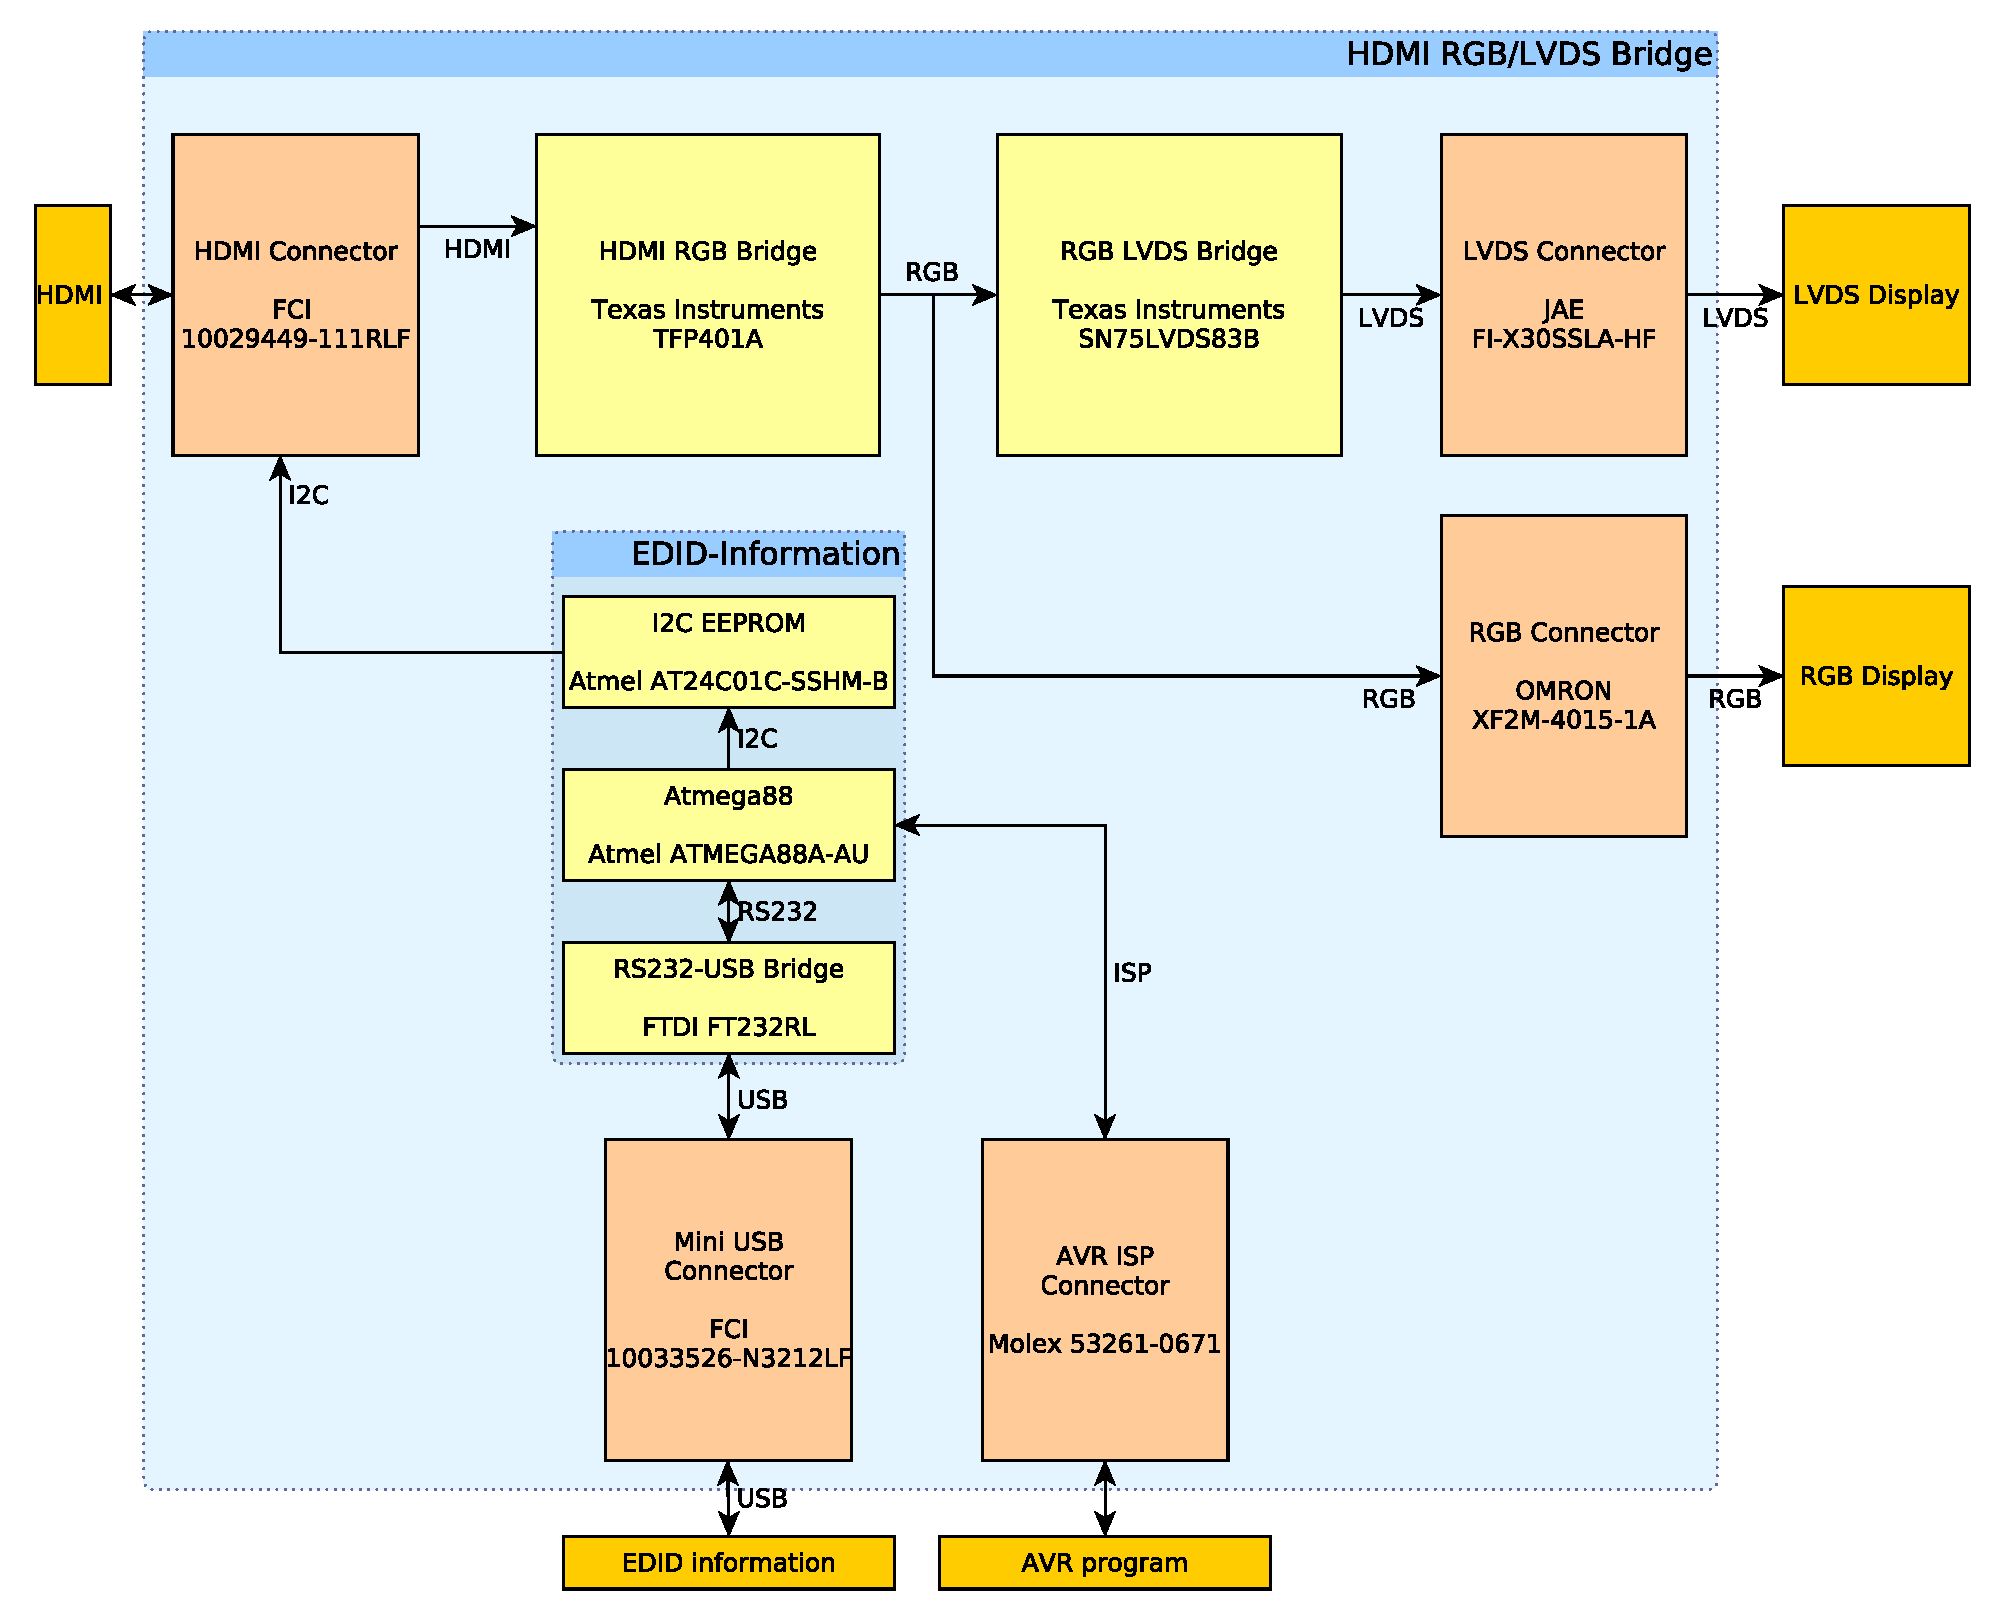
\includegraphics[width=1.0\textwidth]{TeilB/Architektur.pdf}}
	\caption{Hardware-Architektur}
	\label{fig:teilb_architektur}
\end{figure}

\refa{fig:teilb_architektur} zeigt die komplette Architektur des Projekts mit allen notwendigen Eckpunkten und Verbindungen. So sind Schnittstellen nach außen mit rot und die interne Logik mit gelb markiert. Als Signalquelle wird das HDMI-Signal eingespeist und in die \code{HDMI-RGB-Bridge} geleitet. Der Baustein \code{TFP401A} konvertiert die eingehenden HDMI-Signale zum RGB-Bus. Hier kann direkt über einen FPC-Stecker\footnote{FPC: Fine Pitch Connector} ein RGB-Display anschlossen werden. Die Leitungen werden zu einer RGB-LVDS-Bridge weitergeleitet. Diese wandelt die RGB-Signale in LVDS-Signale entsprechend der benötigten Beschaltung des verwendeten Displays um. Wird die Platine mit einer Quelle verbunden, so tauschen beide Informationen aus. Dabei ließt die Quelle Leistungsdaten bzgl. Auflösung, Timings, etc. aus einem EEPROM  im Anzeigegerät aus. Diese Daten werden als EDID-Daten\footnote{EDID: Extended Display Identification Data} bezeichnet (siehe \cite{edid2000}). Gespeichert werden die EDID-Daten üblicherweise in einem EEPROM\footnote{EEPROM: Electrically Eraseable Programmable Read-Only Memory}, auf welches mit dem $I^2C$-Bus zugegriffen wird. Um das EEPROM mit korrekten Inhalten beschreiben zu können, ist eine Baugruppe mit den Namen \code{EDID-Information} realisiert (siehe \refa{fig:teilb_architektur}). Der verwendete USB-Seriell-Konverter FT232RL kommuniziert mit einem 8-Bit Atmel ATMega88 Prozessor, welcher das $I^2C$-EEPROM direkt beschreiben kann. Um die korrekten EDID-Informationen in das EEPROM zu schreiben ist die zugehörige PC Software zu verwenden (siehe \refc{edid_pc}).\newpage

\section{Hardwareentwicklung}
\label{sec:TeilB_Hardware}

\subsection{Spannungsversorgung}
\subsection{HDMI-RGB-Bridge}
\subsection{RGB-LVDS-Bridge}
\subsection{EDID-Daten}


\section{Software}
\label{sec:TeilB_Software}

\subsection{EDID-Daten auf embedded Seite}
\subsubsection{Konzept}
\subsubsection{Low-Level-Treiber}
\paragraph{UART-Treiber}
\paragraph{I2C-Treiber}
\subsubsection{Programmablauf}

\subsection{EDID-Daten auf PC Seite}
\subsubsection{Konzept}
\subsubsection{GTK GUI mit Glade}
\subsubsection{Programmablauf}

\section{Known Bugs}
Im Rahmen der Entwicklung und mit Fortschreiten des Projekts sind, trotz Reviews der einzelnen Elementen des Projekts, Fehler bekannt geworden, die komplett oder teilweise gelöst oder umgangen wurden. Auf diese Fehler wird in den folgenden Abschnitten eingegangen.
\subsection{Hardware}
Bei der Hardwareentwicklung sind Schaltungstechnisch und bzgl. der erstellten Bauteilbibliothek Fehler aufgetreten. 
\subsubsection{HDMI-Stecker gekreuzt}
\textbf{Problem:} Durch einen Fehler beim Erstellen der HDMI-Buchse CON2 im Schaltplanprogramm \code{Eagle} wurde fälschlicherweise die Belegung des Steckers verwendet. Die Verwendung von normalen HDMI-Kabeln ist daher nicht möglich!\\
\textbf{Workaround:} Alle Signale müssen gekreuzt werden. Hierzu wird ein HDMI-Stecker an ein abgetrenntes Ende eines HDMI-Kabels verbunden. Dazu wird die Belegung entsprechend \refa{fig:hdmi_stecker_problem}\footnote{Quelle: \url{http://upload.wikimedia.org/wikipedia/commons/thumb/4/48/HDMI_Connector_Pinout.svg/1280px-HDMI_Connector_Pinout.svg.png}} gekreuzt.
\begin{figure}[htp]
	\center
	\fbox{\includegraphics[width=0.6\textwidth]{TeilB/hdmi_stecker_problem.png}}
    \caption{Known Bugs: HDMI-Stecker, }
    \label{fig:hdmi_stecker_problem}
\end{figure}\\
%    }}
\textbf{Lösung:} Um das Problem endgültig zu lösen, muss das Schaltplansymbol in \code{Eagle} sowie das Platinenlayout bzgl. der Beschaltung der HDMI-Buchse und der RGB-Bridge angepasst werden.
\subsubsection{LVDS-Steckerfootprint gespiegelt}
\textbf{Problem:} Das Schaltplansymbol des LVDS-Steckers CON6 muss gespiegelt werden. Das Anstecken des LVDS-Displays mit vorgesehener Belegung kann zur Zerstörung des Displays führen.\\
\textbf{Workaround:} Der LVDS-Stecker wird um 180 Grad gedreht auf die bereits dort vorgesehenen Pads angelötet.\\
\textbf{Lösung:} Das Schaltplansymbol muss in \code{Eagle} um 180 Grad gedreht werden.
\subsubsection{+5V-Kreis / Widerstand}
\textbf{Problem:} Der Widerstand \code{R13} wird verwendet um eventuell auftretende Spannungsunterschiede zwischen den +5\,V der USB- und HDMI-Versorgung auszugleichen (siehe \refa{fig:r13}). Dieser Widerstand ist mit 10\,k$\Omega$ zu groß gewählt.
\begin{figure}[htp]
	\center
	\fbox{\includegraphics[width=0.2\textwidth]{TeilB/r13.png}}
    \caption{Known Bugs: +5V-Kreis}
    \label{fig:r13}
\end{figure}\\
\textbf{Lösung:} Verkleinerung des Widerstands bzw. Entfernen und Brücken von \code{R13} mit 0\,$\Omega$.
\subsubsection{USB D+/D- vertauscht}
\textbf{Problem:} Die USB-Datensignale \code{USB_D+} und \code{USB_D-} sind vertauscht. Dies verhindert die Kommunikation zwischen PC und AVR (siehe \refa{fig:usb_vertauscht}).
\begin{figure}[htp]
	\center
	\fbox{\includegraphics[width=0.45\textwidth]{TeilB/usb_dp_dm.png}}
    \caption{Known Bugs: USB Signale vertauscht}
    \label{fig:usb_vertauscht}
\end{figure}\\
\textbf{Workaround:} Entfernen der 0\,$\Omega$ Widerstände \code{R22} und \code{R23} und kreuzen der Signale mit Fädeldraht.\\
\textbf{Lösung:} Um das Problem endgültig zu beheben, müssen die Signale \code{USB_D+} und \code{USB_D-} im Schaltplan am Baustein \code{FT232RL} getauscht und im Platinenlayout entsprechende Anpassungen gemacht werden.
\subsection{Software}
\textbf{Problem:} Unter bisher ungeklärten Umständen kann es vorkommen, dass die Prüfsumme des ausgelesenen EEPROMs und der im PC-Programm berechneten Software nicht übereinstimmt. \\
\textbf{Workaround:} Ein erneuter Programmiervorgang umgeht das Problem. Die Prüfsummen werden nun korrekt berechnet und verglichen.
\input{Inhalt/TeilB/TeilBZusammenfassung}